%----------------------------------------------------------------------------------------
%	PACKAGES AND OTHER DOCUMENT CONFIGURATIONS
%----------------------------------------------------------------------------------------

\documentclass[
10pt, % Main document font size
a4paper, % Paper type, use 'letterpaper' for US Letter paper
oneside, % One page layout (no page indentation)
%twoside, % Two page layout (page indentation for binding and different headers)
headinclude,footinclude, % Extra spacing for the header and footer
BCOR5mm, % Binding correction
]{scrartcl}


%%%%%%%%%%%%%%%%%%%%%%%%%%%%%%%%%%%%%%%%%
% Arsclassica Article
% Structure Specification File
%
% This file has been downloaded from:
% http://www.LaTeXTemplates.com
%
% Original author:
% Lorenzo Pantieri (http://www.lorenzopantieri.net) with extensive modifications by:
% Vel (vel@latextemplates.com)
%
% License:
% CC BY-NC-SA 3.0 (http://creativecommons.org/licenses/by-nc-sa/3.0/)
%
%%%%%%%%%%%%%%%%%%%%%%%%%%%%%%%%%%%%%%%%%

%----------------------------------------------------------------------------------------
%	REQUIRED PACKAGES
%----------------------------------------------------------------------------------------

\usepackage[
nochapters, % Turn off chapters since this is an article        
beramono, % Use the Bera Mono font for monospaced text (\texttt)
eulermath,% Use the Euler font for mathematics
pdfspacing, % Makes use of pdftex’ letter spacing capabilities via the microtype package
dottedtoc % Dotted lines leading to the page numbers in the table of contents
]{classicthesis} % The layout is based on the Classic Thesis style

\usepackage{arsclassica} % Modifies the Classic Thesis package

\usepackage[T1]{fontenc} % Use 8-bit encoding that has 256 glyphs

\usepackage[utf8]{inputenc} % Required for including letters with accents

\usepackage{graphicx} % Required for including images
\graphicspath{{Figures/}} % Set the default folder for images

\usepackage{enumitem} % Required for manipulating the whitespace between and within lists

\usepackage{lipsum} % Used for inserting dummy 'Lorem ipsum' text into the template

\usepackage{subfig} % Required for creating figures with multiple parts (subfigures)

\usepackage{amsmath,amssymb,amsthm} % For including math equations, theorems, symbols, etc

\usepackage{varioref} % More descriptive referencing

\usepackage{amsmath}

\usepackage{tcolorbox}

\tcbuselibrary{theorems}

\newtcbtheorem[]{mydef}{Definition}%
{colback=white!5,colframe=black!35!black,fonttitle=\bfseries}{def}


%----------------------------------------------------------------------------------------
%	THEOREM STYLES
%---------------------------------------------------------------------------------------

\theoremstyle{definition} % Define theorem styles here based on the definition style (used for definitions and examples)
\newtheorem{definition}{Definition}

\theoremstyle{plain} % Define theorem styles here based on the plain style (used for theorems, lemmas, propositions)
\newtheorem{theorem}{Theorem}

\theoremstyle{remark} % Define theorem styles here based on the remark style (used for remarks and notes)

%----------------------------------------------------------------------------------------
%	HYPERLINKS
%---------------------------------------------------------------------------------------

\hypersetup{
%draft, % Uncomment to remove all links (useful for printing in black and white)
colorlinks=true, breaklinks=true, bookmarks=true,bookmarksnumbered,
urlcolor=webbrown, linkcolor=RoyalBlue, citecolor=webgreen, % Link colors
pdftitle={}, % PDF title
pdfauthor={\textcopyright}, % PDF Author
pdfsubject={}, % PDF Subject
pdfkeywords={}, % PDF Keywords
pdfcreator={pdfLaTeX}, % PDF Creator
pdfproducer={LaTeX with hyperref and ClassicThesis} % PDF producer
} % Include the structure.tex file which specified the document structure and layout

\usepackage{amsmath}

\hyphenation{Fortran hy-phen-ation} % Specify custom hyphenation points in words with dashes where you would like hyphenation to occur, or alternatively, don't put any dashes in a word to stop hyphenation altogether

%----------------------------------------------------------------------------------------
%	TITLE AND AUTHOR(S)
%----------------------------------------------------------------------------------------

\title{\normalfont\spacedallcaps{SEARCHING NUTRIENT PREFERENCE ON NETWORK TOPOLOGY}} % The article title

\subtitle{(not a paper draft)} % Uncomment to display a subtitle

% \author{\spacedlowsmallcaps{John Smith* \& James Smith\textsuperscript{1}}} % The article author(s) - author affiliations need to be specified in the AUTHOR AFFILIATIONS block

\date{} % An optional date to appear under the author(s)

%----------------------------------------------------------------------------------------

\begin{document}

%----------------------------------------------------------------------------------------
%	HEADERS
%----------------------------------------------------------------------------------------

\renewcommand{\sectionmark}[1]{\markright{\spacedlowsmallcaps{#1}}} % The header for all pages (oneside) or for even pages (twoside)
%\renewcommand{\subsectionmark}[1]{\markright{\thesubsection~#1}} % Uncomment when using the twoside option - this modifies the header on odd pages
\lehead{\mbox{\llap{\small\thepage\kern1em\color{halfgray} \vline}\color{halfgray}\hspace{0.5em}\rightmark\hfil}} % The header style

\pagestyle{scrheadings} % Enable the headers specified in this block

\maketitle % Print the title/author/date block

\setcounter{tocdepth}{2} % Set the depth of the table of contents to show sections and subsections only

%----------------------------------------------------------------------------------------
%	MODELS
%----------------------------------------------------------------------------------------

\section{E. COLI NUTRIENT PREFERENCES}
\label{sec:ecoli_nut_preference}

It is found that E. coli has preferences at the time to consume nutrients in a complex medium.
For instance, even when several carbon sources are available E. coli might consume only one nutrient till its depletion, and only later, start to consume others. 
The sequence of consumption is reproducible. 

Figures \ref{fig:begIntracellularCrowdingDefines2007a_carbon_evolution} and \ref{fig:maserAvoidingAminoAcid2019_aa_sequence}
show two examples.

\begin{figure}[h]
    \centering
    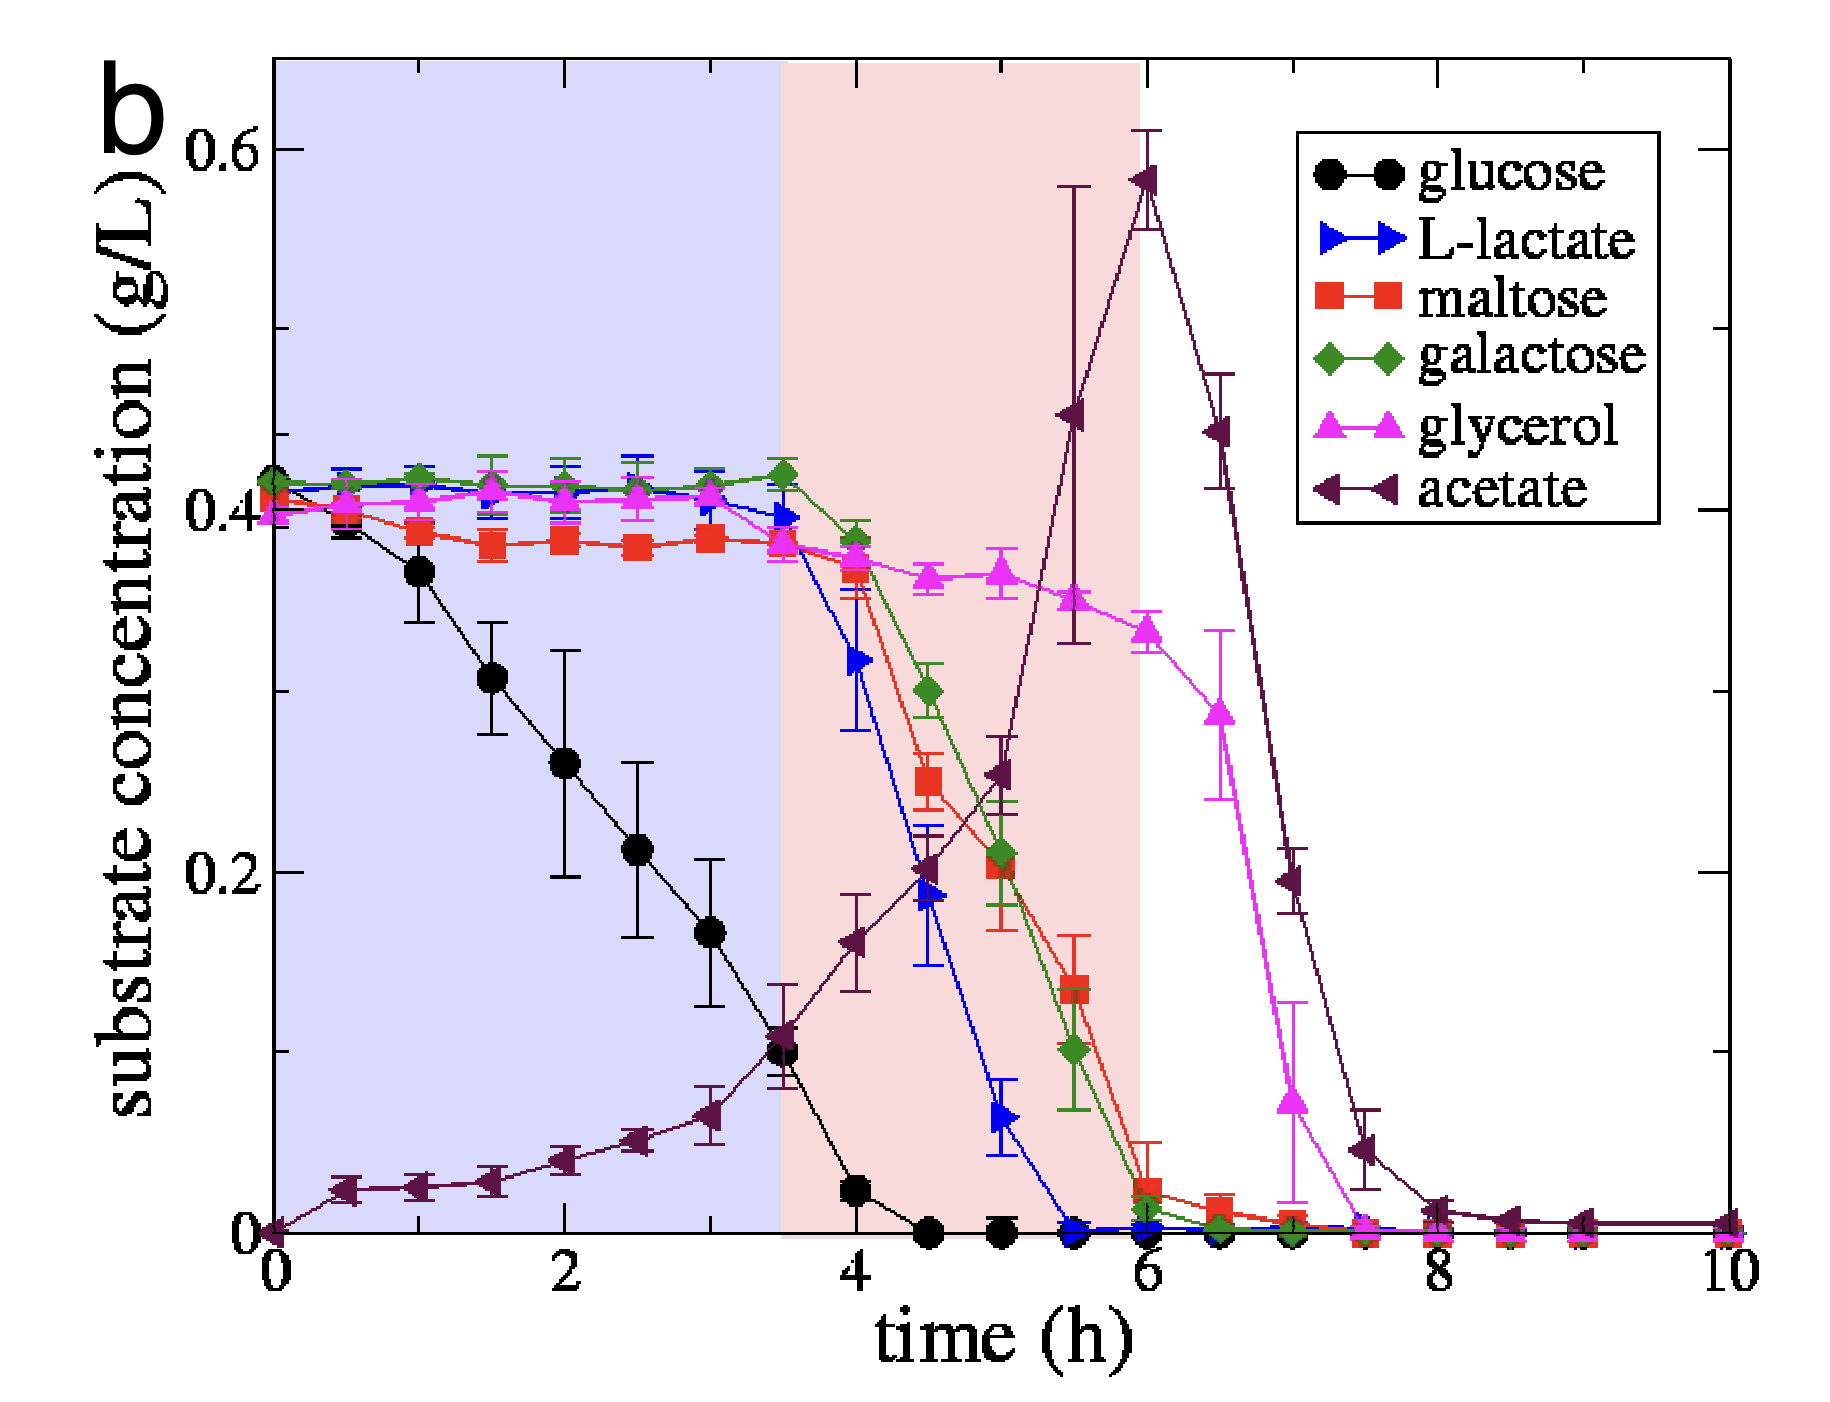
\includegraphics[width=0.8\columnwidth]{images/begIntracellularCrowdingDefines2007a_carbon_evolution.png}
    \caption[]{
        Time evolution of the concentration of several nutrients (plus acetate) present in the medium of an E. coli batch culture. 
        Taken without request from \cite{begIntracellularCrowdingDefines2007a}.
    }
    \label{fig:begIntracellularCrowdingDefines2007a_carbon_evolution}
\end{figure}

\begin{figure}[h]
    \centering
    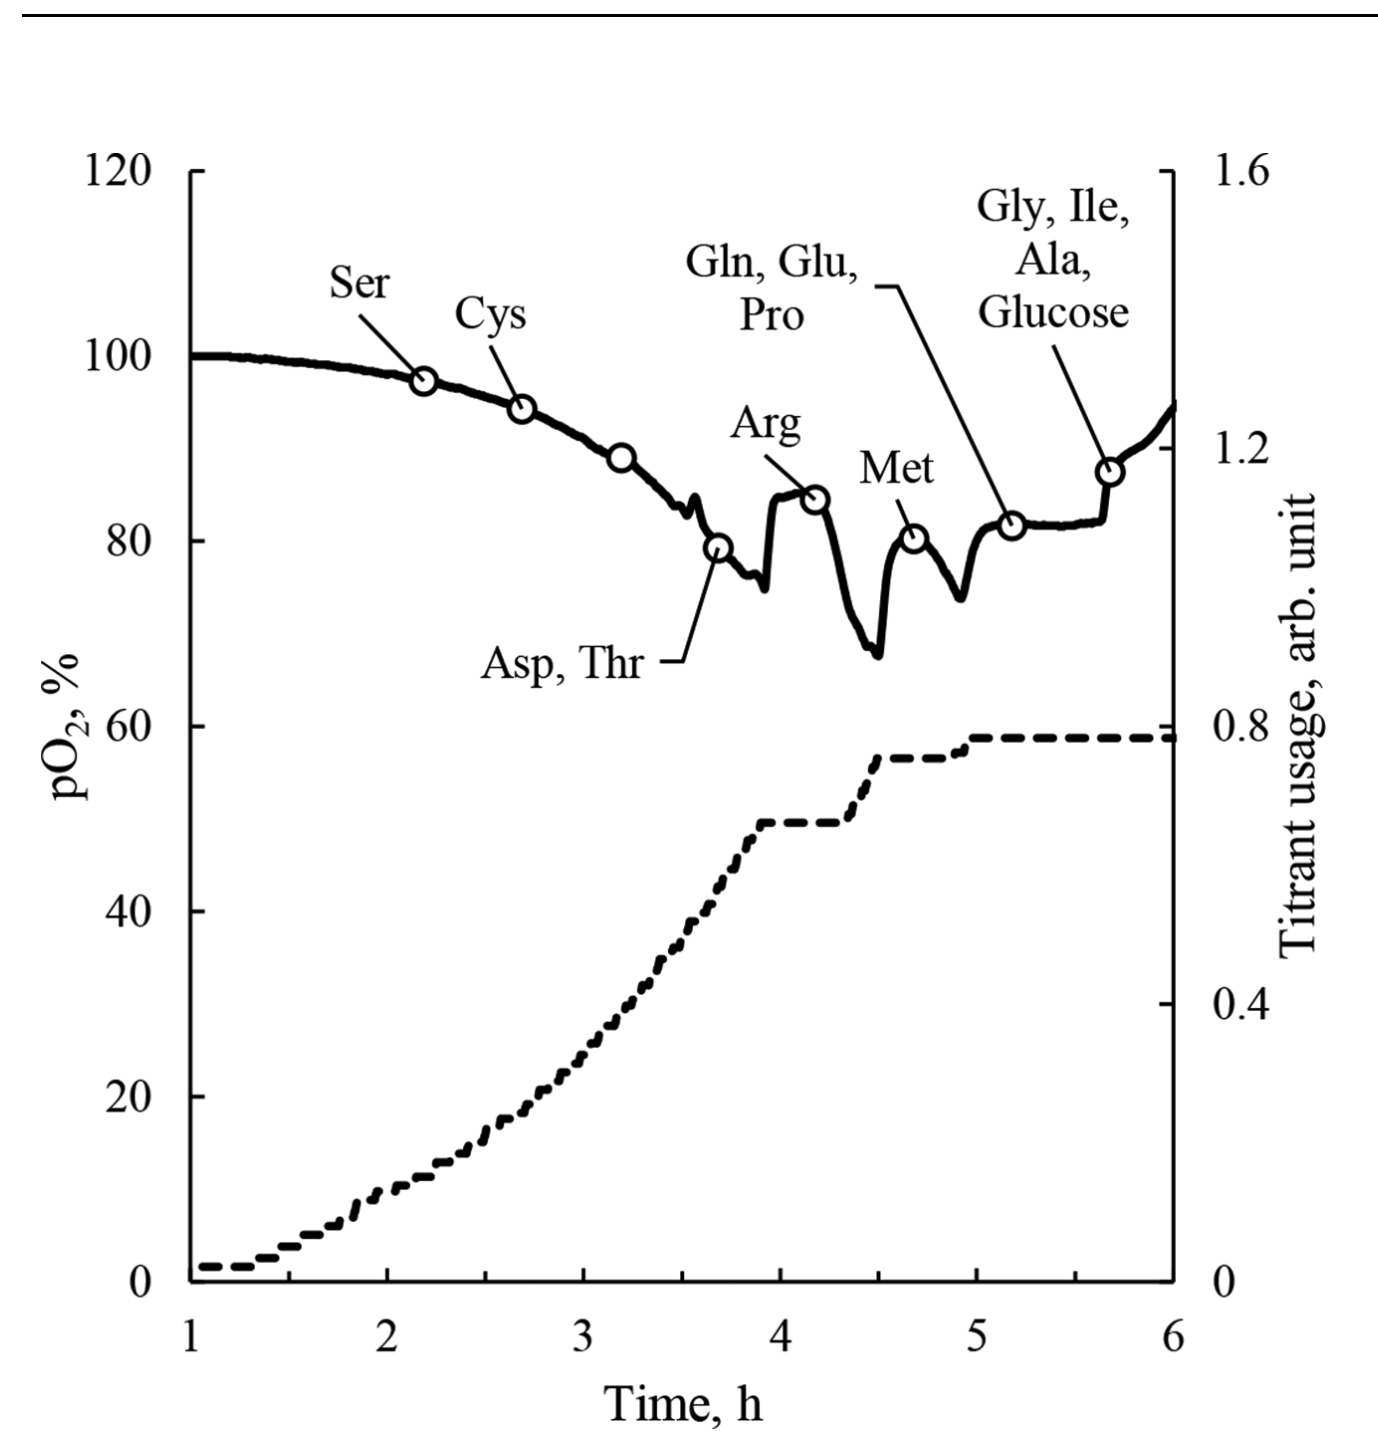
\includegraphics[width=0.8\columnwidth]{images/maserAvoidingAminoAcid2019_aa_sequence.png}
    \caption[]{
        Ignore the lines and the vertical axis. 
        The empty circles mark the moment when the labeled nutrients were depleted in an E. coli batch culture.
        Taken without request from \cite{maserAvoidingAminoAcid2019}.
    }
    \label{fig:maserAvoidingAminoAcid2019_aa_sequence}
\end{figure}


\section{TOPOLOGICAL PREFERENCE}

Because we are very brave, we will try to find if the topology of the network do contain biases which are conherent with the nutrient expeimental preferences. 
The cell can control its metabolic configuration using several regulatory stratergies. We can not explore must of this regulatory space, which includes alosteric, equilibrium, expression and localization regulation, among others. 
But, we can try to explore one of the consequences of such regulation events, a flux knockout (KO).
Given a network with $N$ independent variables, the space of KO's contain $2^N$ KO sequences.
For a typical genome scale metabolic network, this number is very big ($> 10^{180}$ for E. coli).
This makes any computation exploring such space unfeasible. 
Luckly, we hope, not all KO sequences are interesting. 
Because the network is well connected, very large KO sequences (a set of many blocked reactions) are expected to affect important network properties like the posibility to growth from the medium. 
This is our hope, that the feasible KO space is not prohibited big.

Once we can explore the feasible space of KO configurations, we can compare the configurations dependency on all nutrients of interest.
For instance, we can characterize the average number of KO required for the network to have glucose as an essential nutrient.
Or we can count how many of such networks there are. 
By comparing such measurements between nutrient, we can argue we are computing the relative bias toward a given nutrinet present in the topology of the network.
Note that, for now, we are only taking into consideration the connectivity of the network, not the stoichiometry (eg. shadow prices). 

\section{WIP, SOME RESULTS: KOMC}

At the cluster we are running a Monte Carlos exploring the KO space for the genome scale network of E. coli iJO1366 (metabolites $1110$, reactions $1694$, free reactions $584$) \cite{orthComprehensiveGenomescaleReconstruction2011}.
Right now we are just computing the limits of the feasible space (finding KO sequences which are fatal).
Here we are presenting the results for the first 550011 samples for the medium described at Figure \ref{fig:begIntracellularCrowdingDefines2007a_carbon_evolution} reference. 
I have not completed the scripts for evaluating nutrient essentiality yet. So, I'll present only some statistics of the KO samples. 

\begin{figure}[h]
    \centering
    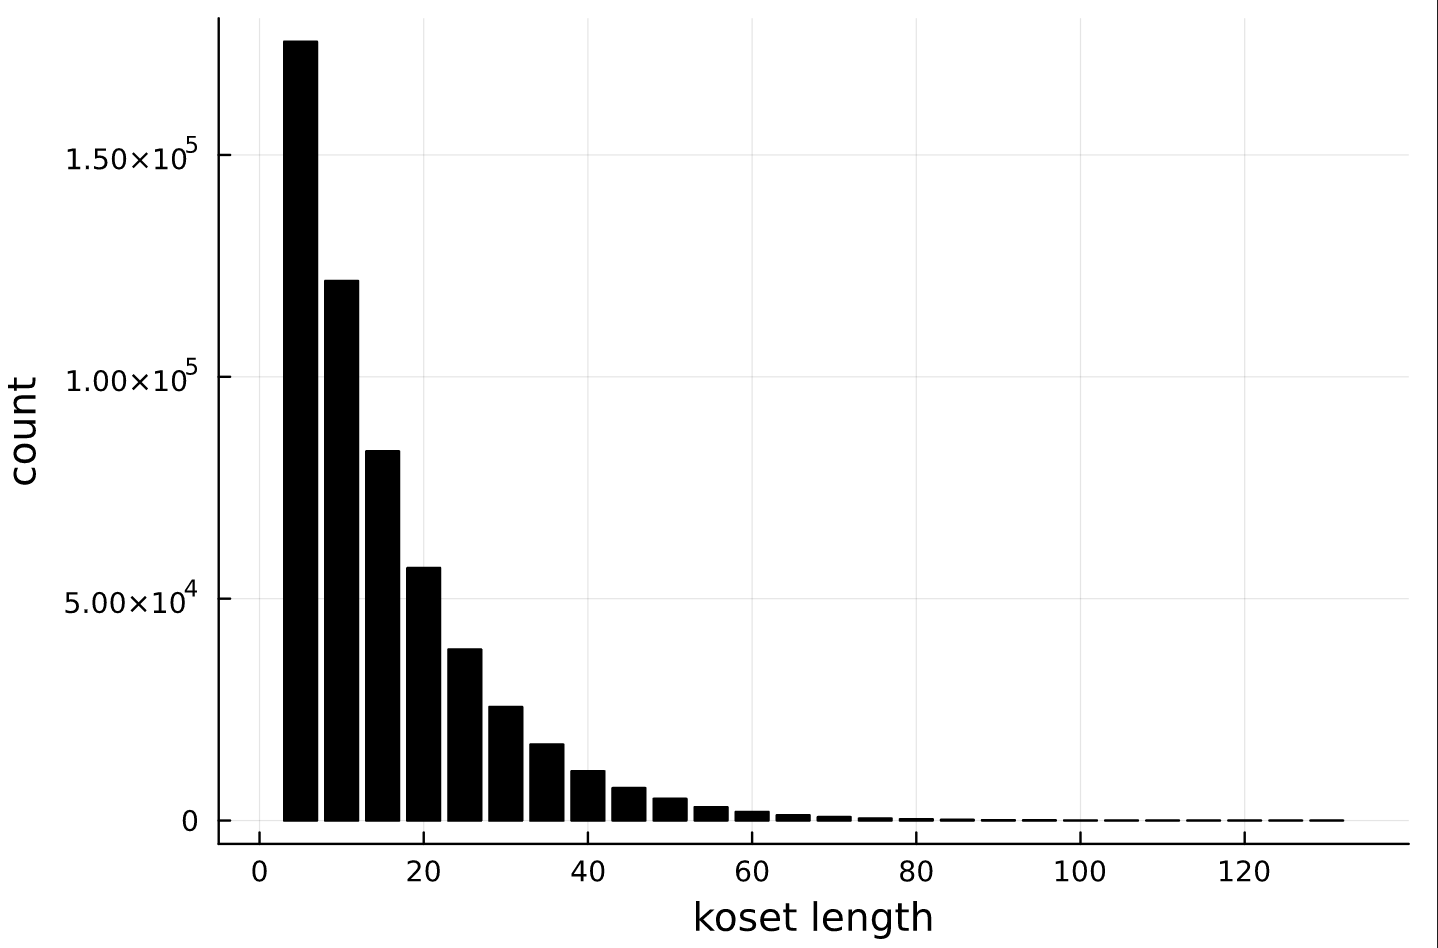
\includegraphics[width=0.8\columnwidth]{images/kosets_length.png}
    \caption[]{Histogram of the lenghts of KO sequences for 550011 MC samples. }
    \label{fig:kosets_length}
\end{figure}

Figure \ref{fig:kosets_length} shows the distributions of the lenghts of the KO sequences. 
A $20$ means that $20$ reactions were blocked before the network was unable to produce biomass.

\begin{figure}[h]
    \centering
    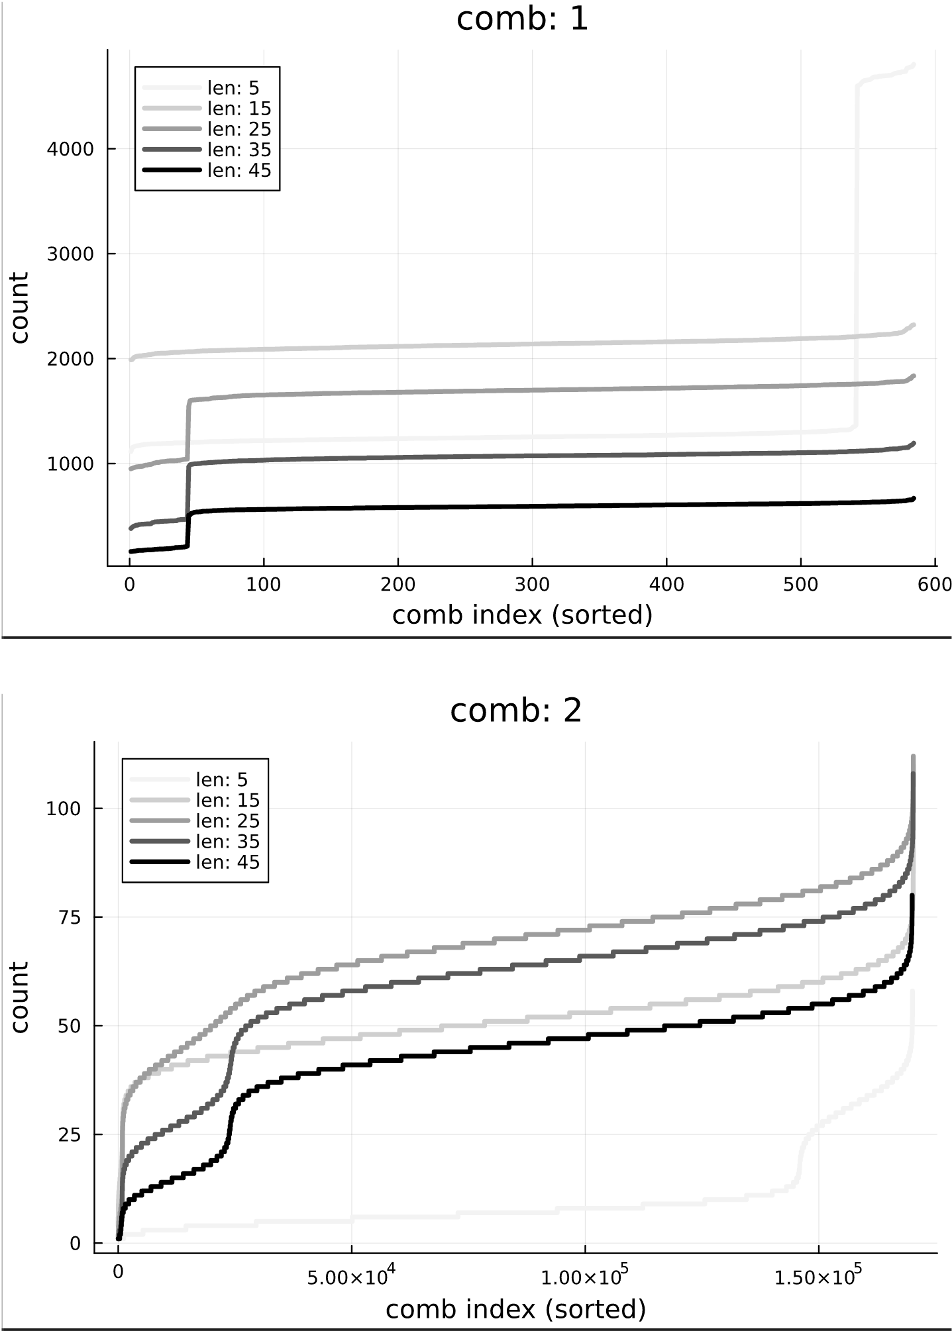
\includegraphics[width=0.8\columnwidth]{images/KOMC_comb1-2.png}
    \caption[]{Histogram of the count of each reactions and pair of reactions for 550011 unfeasible KO samples.}
    \label{fig:KOMC_comb1-2}
\end{figure}

Figure \ref{fig:KOMC_comb1-2} shows the histogram for the single reaction combinatory (the count of each reaction on the KO configurations), 
and the two reaction combinatory (the count of each pair of reactions).
In the first panel (top) we can clearly see the fatal single KOs, they are very common at shorter KO sets, and less common at the larger. 
This is obious, short KO sets can mostly be so it they contain a very fatal limitation, for large KO sets is the oposite, if they contain them it can only be one after many non fatal reactions.
Note that the x axis are just an enumeration of the elements (reactions or pair of reactions) and aren't the same for each line (beacuase of plotting considerations).
That is, at Figure \ref{fig:KOMC_comb1-2} we are only studying the shape of the histograms.

At the momment, the main questions are: How close to equilibrium is the MC? How much time we should keep running it? It is feasible?


\section{SUMMARY}

Computations are probably unfeasible, questions aren't clear, data non available or noisy, rewards not very promising.
Unfortunately, just like 7 months ago.


% For us, this is important because that saids something about $c$ itself (that is "large") 


% Actuatlly, the authors did growth the cells with and without glycine for comparison (see Figure \ref{fig:gly_cancer_ko}). 
% Glycine became more and more "essental" as the cells displayed a larger proliferation rate.

% \begin{figure}[h]
%    \centering
%    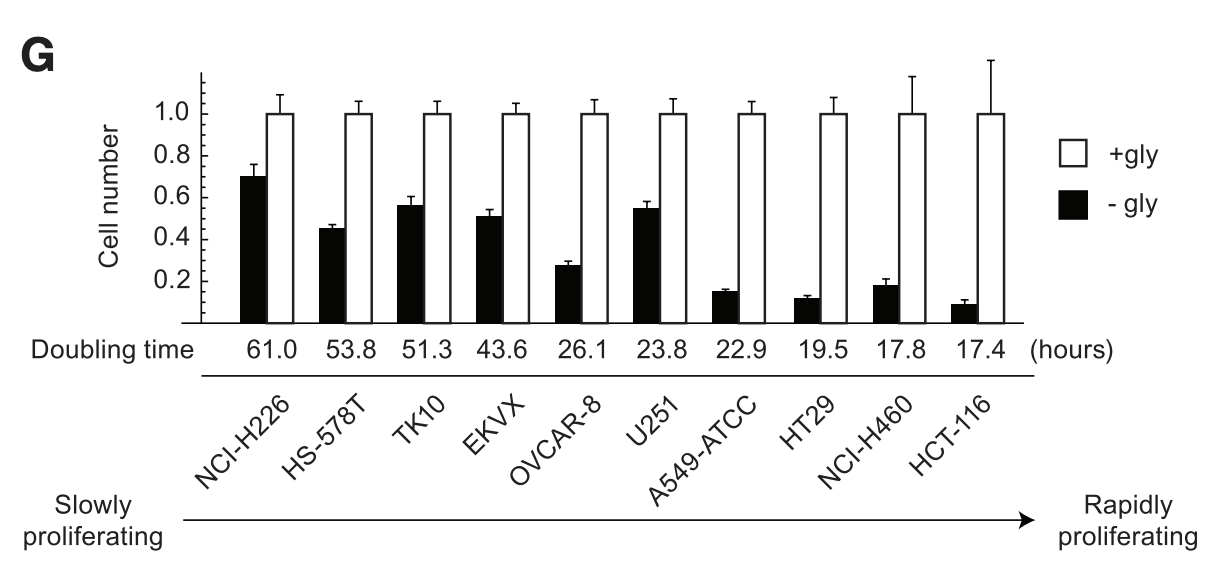
\includegraphics[width=0.8\columnwidth]{images/gly_cancer_ko.png}
%    \caption[]{
%       Reproduced without authorization from \cite{jainMetaboliteProfilingIdentifies2012}.
%    }
%    \label{fig:gly_cancer_ko}
% \end{figure}

% Whenever you find a linear dependency between fluxes, you are in an edge of the polytope?.






% First, let define the set of exchage reactions (the prefix $Ex\_$ denotes exchange), which input matter into the model. 
% \begin{itemize}[label=$$]
%    \item Exchange reactions
%    \begin{itemize}[label=$$]
%       \item $Ex\_A$:   $(-1)~A \Leftarrow$
%       \item $Ex\_E$: $(-1)~E \Leftarrow$
%       \item $Ex\_S$: $(-1)~S \Leftarrow$
%    \end{itemize}
% \end{itemize}

% Where: 
% Metabolite $E$ is an always essential metabolite.
% Metabolite $S$ is a non necesarilly essential metabolite.
% And $A$ is just a particular metabolite which is the focus of the analisis.

% Second, the biomass reaction is the sink of matter from the model.
% \begin{itemize}[label=$$]
%    \item Biomass equation
%    \begin{itemize}[label=$$]
%       \item $z$: $ (-1)E + (-1)P_1 + (-1)P_2 \Rightarrow$
%    \end{itemize}
% \end{itemize}


% Where: Metabolites $P_{*}$ are internal metabolites. 

% Finally, the internal reactions are the source of degeneracy of the system. 
% They introduce an exponentialy growing combinations of routes for matter to flow from the inputs (exchanges) to the sink (biomass).

% \begin{itemize}[label=$$]
%    \item Internal reactions

%    \begin{itemize}[label=$$]
%       \item $(-1)S \Rightarrow P_1$
%       \item $(-1)S \Rightarrow P_2$
%       \item $(-1)A \Rightarrow P_1$
%       \item $(-1)A \Rightarrow P_2$
%    \end{itemize}
% \end{itemize}

% Here we are considering each reaction as a total reaction (eg. $(-1)S \Rightarrow N P_1$ means that exist an open route from $S$ to $P_1$).

% Note that in the current configuration, assumming all exchanges are unbounded, the metabolite $A$ is neither limiting no essenctial.
% That is, the components of the biomass can be acquired from $S$.
% This situation can change if we do the follow transformations on the network:
% \begin{itemize}[label=$$]
   
%    \item i) Make $A$ essential: knocking the connections of $S$ to at least one component of $z$ which, at the same time, is reachable from $A$. For instance:
%    \begin{itemize}[label=$$]
%       \item Blocking $(-1)S \Rightarrow P_1$ will make $A$ the only source of $P_1$
%    \end{itemize}

%    \item ii) Create a bottleneck: If we limit (not block) the connection from $S$ to components of $z$, there will be always a regime of $z$ for which
%    $A$ is limiting. The case (i) is just an extreme of this one (where the regime of $z$ is all reals).
%    For instance: 
%    \begin{itemize}[label=$$]
%       \item If we limit $(-1)S \Rightarrow P_1$ so not all $P_1$ required for $z > C$ can be produced from $S$, 
%       $(-1)A \Rightarrow P_1$ will must the gap, and so, above this threshold, $z$ will depend on $Ex\_A$.
%    \end{itemize}
   
%    \item iii) Reduce the yield of $A$ under a defined medium: Here, reactions are blocked so the total ones (eg. $(-1)A \Rightarrow P_1$) reduces it yeild 
%    (eg. number of $P_1$ per $A$ produced, stoichiometric coefficients aren't shown). This can lead to the requirements of $z$ being to higt for 
%    the amount of $A$ and $S$ available in the deffined medium. This is different of the case (ii) because now we are not limiting the network capacity of 
%    consuming a nutrient, we are making it so ineficient that a previously suffitient resource become limiting.
   
%    \item iv) A combination of the previous

% \end{itemize}


% An important difference between the alternatives are the combinational space they produces (we will ignore (iv)). 
% The alternatives (i and ii) can be realized by exploring up to $2^{no. reactions}$ combinations.
% One per each KO/reduction pattern over the network. 

% \subsection{REDUCE THE COMBINATIONAL SPACE}




% \subsection{GENERAL MODEL}

% First, let define the set of exchage reactions (the prefix $Ex\_$ denotes exchange), which input matter into the model. 
% \begin{itemize}
%    \item Exchange reactions
%    \begin{itemize}
%       \item $Ex\_A$:   $(-1)~A \Leftarrow$
%       \item $Ex\_E_e$: $(-1)~E_e \Leftarrow$
%       \item $Ex\_S_s$: $(-1)~S_s \Leftarrow$
%    \end{itemize}
% \end{itemize}

% Where: 
% The set of metabolites $E_e$, $e \in [1,M_E]$, are the essential metabolites.
% The set of metabolites $S_s$, $s \in [1,M_S]$, are the non-essential metabolites.
% And $A$ is just a particular metabolite which is the target of the analisis.

% Second, the biomass reaction is the sink of matter from the model.

% \begin{itemize}
%    \item Biomass

%    \begin{itemize}
%       \item $z$:   $ \sum^{M_E} S_{ze} E_e + \sum^{M_S} S_{zs} E_s + S_{zA} A\Rightarrow$
%    \end{itemize}
% \end{itemize}

% The stoichiometric coefficients ($c_{*}$) control whom ultimatly is a biomass component. 

% Finally, the internal reactions are the source of degeneracy of the system. 
% They introduce an exponentialy growing combinations of routes for matter to flow from the inputs (exchanges) to the sink (biomass).
% We aim at 

% \begin{itemize}
%    \item Internal reactions

%    \begin{itemize}
%       \item $r_j$: $ \sum S_{ej} E_e \Rightarrow$
%    \end{itemize}
% \end{itemize}


































%----------------------------------------------------------------------------------------
%	BIBLIOGRAPHY
%----------------------------------------------------------------------------------------

\renewcommand{\refname}{\spacedlowsmallcaps{References}} % For modifying the bibliography heading

\bibliographystyle{unsrt}

\bibliography{report.bib} % The file containing the bibliography

%----------------------------------------------------------------------------------------

\end{document}